\section{Results}
\label{sec:results}

We trained our model for 40 epochs and the loss greatly reduced from 1.0 to 0.3. The reduction in loss after the 40th epoch was neglegible. The performance of model is tested using the following metrics: epoch loss, pixel accuracy, IoU score, Dice score, and F1 score. The model achieved 88.52\% pixel accuracy (cumulative for all classes) after training on train set. IoU score, Dice score, and F1 score values for train set can be found in Table 1. The pixel accuracy on test set is 81.85\%. IoU score, Dice score, and F1 score values fort test set can be found in Table 2. We can see, from the plots, the model performs best on the background class, followed by the muscle layer class, electrode class and mucosal layer class. The high difference between the metric values of classes indicated high bias in our data.

\begin{table}[htbp]
    \centering
    \caption{Train set performance metrics}
    \label{tab:train-metrics}

    \begin{tabular}{|c|c|c|}
        \hline
        & \textbf{Background} & \textbf{Muscle layer} \\
        \hline
        \textbf{IoU score} & 0.8312 & 0.6159 \\
        \textbf{Dice score} & 0.4528 & 0.3423 \\
        \textbf{F1 score} & 0.9056 & 0.6846 \\
        \hline
    \end{tabular}

    \begin{tabular}{|c|c|c|}
        \hline
        & \textbf{Mucosal layer} & \textbf{Electrode} \\
        \hline
        \textbf{IoU score} & 0.2282 & 0.4474 \\
        \textbf{Dice score} & 0.1339 & 0.2656 \\
        \textbf{F1 score} & 0.2678 & 0.5312 \\
        \hline
    \end{tabular}

\end{table}

\begin{table}[htbp]
    \centering
    \caption{Test set performance metrics}
    \label{tab:test-metrics}

    \begin{tabular}{|c|c|c|}
        \hline
        & \textbf{Background} & \textbf{Muscle layer} \\
        \hline
        \textbf{IoU score} & 0.7733 & 0.4744 \\
        \textbf{Dice score} & 0.4338 & 0.2735 \\
        \textbf{F1 score} & 0.8677 & 0.5470 \\
        \hline
    \end{tabular}

    \begin{tabular}{|c|c|c|}
        \hline
        & \textbf{Mucosal layer} & \textbf{Electrode} \\
        \hline
        \textbf{IoU score} & 0.2081 & 0.3466 \\
        \textbf{Dice score} & 0.1314 & 0.2167 \\
        \textbf{F1 score} & 0.2628 & 0.4334 \\
        \hline
    \end{tabular}

\end{table}

\begin{figure}[htp!]
    \centering
    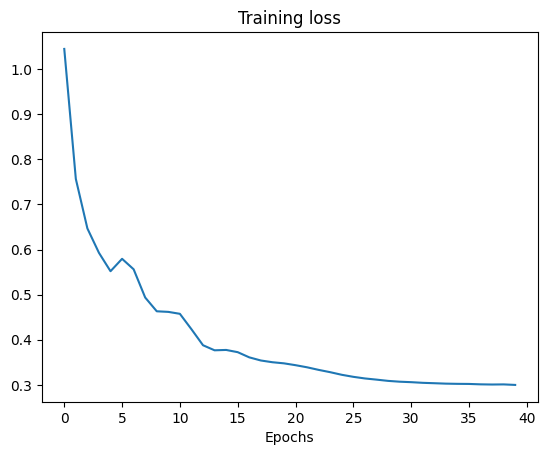
\includegraphics[width=0.4\textwidth]{Images/loss.png}
    \caption{MobileNetV3 training loss}
    \label{fig:loss}
\end{figure}

\begin{figure}[htp!]
    \centering
    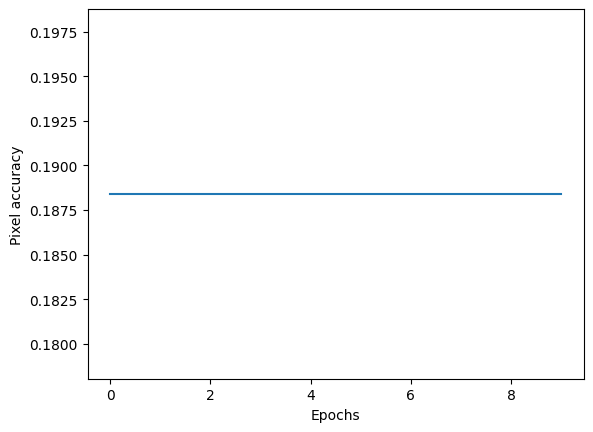
\includegraphics[width=0.4\textwidth]{Images/accuracy.png}
    \caption{MobileNetV3 pixel accuracy}
    \label{fig:accuracy}
\end{figure}

\begin{figure}[htp!]
    \centering
    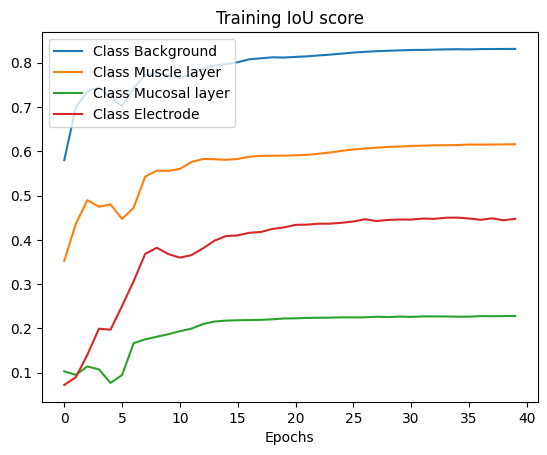
\includegraphics[width=0.4\textwidth]{Images/iou.png}
    \caption{MobileNetV3 IoU score}
    \label{fig:iou}
\end{figure}

\begin{figure}[htp!]
    \centering
    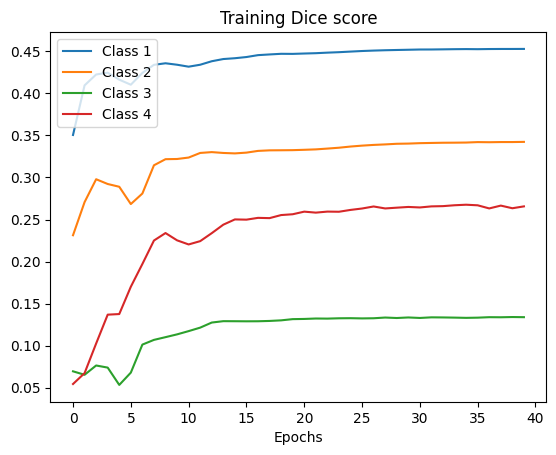
\includegraphics[width=0.4\textwidth]{Images/dice.png}
    \caption{MobileNetV3 dice score}
    \label{fig:dice}
\end{figure}

\begin{figure}[htp!]
    \centering
    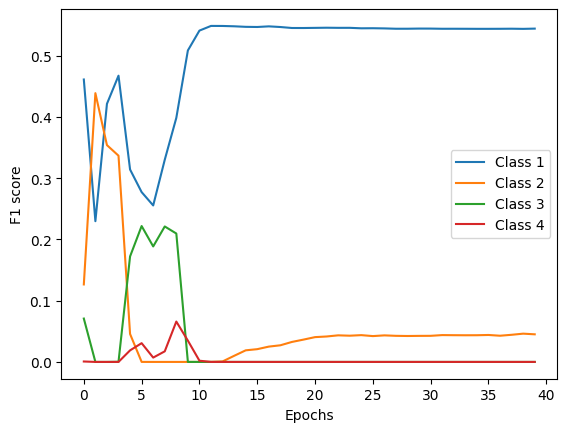
\includegraphics[width=0.4\textwidth]{Images/f1.png}
    \caption{MobileNetV3 F1 score}
    \label{fig:f1}
\end{figure}
